\documentclass[oneside,letterpaper]{memoir}


\setlength{\parindent}{0pt}
\usepackage[margin=1in]{geometry}
\geometry{letterpaper}                   	
\usepackage{graphicx}				
\usepackage{amssymb}
\usepackage{amsmath}
\usepackage{commath}
\usepackage{physics}
\usepackage[utf8]{inputenc}
\usepackage{amsthm}
\usepackage[english]{babel}
\usepackage{graphicx}
\usepackage{blkarray}
\usepackage{mathtools}
\usepackage{listings}
\usepackage{algorithm2e}
\usepackage{tikz}
\usetikzlibrary{arrows,automata,positioning}

\usepackage{prooftrees} %The trees n things!

\newtheorem{proposition}{Proposition}
\newtheorem{theorem}{Theorem}
\newtheorem{corollary}{Corollary}[theorem]
\newtheorem{lemma}[theorem]{Lemma}

\theoremstyle{definition}
\newtheorem*{definition}{Definition}
\newtheorem*{remark}{Remark}
\newtheorem{example}{Example}

\DeclareMathOperator{\ran}{\text{ran }} %% Needed in Aug12_2016
\DeclareMathOperator{\im}{\text{im }}
\DeclareMathOperator{\tand}{\text{ and }}
\DeclareMathOperator{\tor}{\text{ or }}
\DeclareMathOperator{\lt}{<}
%\DeclareMathOperator{\inv}/toolazy

\title{PHIL 379 - Logic II}
\date{Winter 2016}
\author{Scott Saunders - 10163541}

\begin{document}
\maketitle
%\newpage
%Jan 10, 2017.

\subsection{Misc. Notation}

\begin{itemize}
\item The set of positive integers $\{ x : x$ is a positive integer $\}$ 
\item The set of positive integers less than3 $\{ x : x $ is a positive integer and x is less than 3 $\}$. $= \{1,2\}$. 
%I'm already bored.
\item The empty set: $\emptyset \tor \Delta$ 
\item Member of: $A \subseteq B$ iff $\forall X (x \in A \implies x \in B )$ 
\item Union of A and B: $A \cup B $ iff $\{ x : x \in A \lor x \in B \}$
\item Intersection of A and B: $A \cap B $ iff $\{ x : x \in A \land x \in B \}$
\item Difference of A and B: $\{ x : x \in A \land x \not \in B \}$
\item For any non-empty sets $A,B$:
Cartesian product: A of B: $A \cross B$: $\{<x,y>: x \in A \land y \in B \}$ (ALL OF THE POSSIBILITIES)
\item TOTAL FUNCTION: Every element in the domain is valid
\item PARTIAL FUNCTION: Not every element in the domain is valid.
%%LEC02:
\item for any set of sets $A$:
\begin{itemize}
\item $\Cup A = \{ x : \exists y ( y \in A \land x \in y ) \}$ 
\item $\Cap A = \{ x : \forall y (y \in A \to x \in y )\}$ 
\end{itemize}
%%OHBOYTHESEAGAIN
\item Relations: R is 
\begin{itemize}
\item reflexive : $\forall x Rxx$
\item symmetric : $\forall x \forall y (Rxy \implies Ryx)$
\item transitive : $\forall x \forall y \forall z ((Rxy \land Ryz) \implies Rxz)$
\item Euclidean : $\forall x \forall y \forall z ((Rxy \land Rxz ) \implies Ryz)$
\item a equivalence relation : it's symmetric,reflexive,transitive.
\item a equivalence relation (alt) : it's symmetric, and euclidean.
\item a (partial) function : $\exists x$ and there is at most one y: $Rxy$ : denoted $f$
\item a (partial) function$^{1}$ :  $\exists x , \exists y | Rxy$ : denoted $f$.
\item a (total) function: assigns a value to each number of $A$ : denoted $f$
%\item a inverse function: if $\forall x $...?
\item a (total) function$^{2}$: $\forall x , \exists y | Rxy$: denoted $f$.

\end{itemize}

\item Domain: The set of a functions arguments. 
\item Range: The set of its values. (Results) 
\item $f$ is a function from a set $A$ iff the domain of $f$ is included in $A$ 

\item $f$ is a function to a set $B$ iff its range is included in $B$. 
%\item $f$ is a total function of a set $A$ iff $f$ assigns a value to each number of $A$.

\item $f^{-1}$ is the inverse of the function $f$ from the set $A$ to the set $B$ iff:if for every member $b \in B$, there is exactly one member of $a \in A$ such that $f(a)=b$, then $f^{-1}(b)=a$, otherwise $f^{-1}(b)$ is undefined.

\item $f$ is onto $B$ iff $B$ is the range of $f$ (Surjective) \\ 
Alt: (Wikipedia) : $\forall y \in Y, \exists x \in X | y=f(x)$
\item $f$ is one-to-one iff $\forall x \forall y (f(x)=f(y)\implies x=y)$ (Injective)
\item $f$ is a bijection iff $f$ is onto and one-to-one.
\item $f$ is a correspondence iff $f$ is total, one-to-one and onto.
\item Sets $A$ and $B$ are equinumerous iff there is a correspondence from $A$ to $B$.% (Isomorphism?-esk)
%Course plan: Review, Do halting problem, compelteness theorem, misc crap.
\end{itemize}


%Lecture 3
\begin{proof}[Equinumerous is transitive]
Prove: if $A$ is equinumerous with $B$ and $B$ is equinumerous wit $C$, then $A$ is equinumerous with $C$.
Proof: Suppose $A$ is equinumerous to $B$, and $B$ is equinumerous to $C$. Then:
There is a total,one-to-one function $f$ from $A$ onto $B$, and a total one-to-one function $g$ from $B$ to $C$.
Prove equinumerous via h=g(f), such that h(n)=g(f(n))
\begin{itemize}
\item h is total: Let $a$ be a member of $A$. $h(a) = g(f(a))$. Since f is total there is a member of $b$ of $B$ such that $f(a)=b)$. since $g$ is total, there is a member of $c \in C$ such that $g(b)=c$. Hence, $h$ is total.
\item $h$ is onto $C$. WLOG Let $c$ be a member of $C$, as $g$ is onto, $\exists b \in B$ such that $g(b)=c$. As $f$ is onto, then $\exists a \in A $ such that $f(a)=b$. Hence, the composition of $h=f(g)$ is onto $C$.
\item $h$ is one-to-one: Suppose $h$ is not one-to-one. \\
Then there $\exists a_1,a_2 \in A$ such that $h(a_1)=h(a_2), a_1 \not = a_2$.\\
Giving $g(f(a_1))=g(f(a_2)), a_1 /not = a_2$\\
Since $g$ is one-to-one $g(b_1) = g(b_2)$ iff $b_1=b_2$. \\
So the issue must lie in $f$.  However $f$ is one-to-one $f(a_1) = f(a_2)$ iff $f(a) = f(b)$.
Which is a contradiction, giving us that $h$ is one-to-one.
\end{itemize}
\end{proof}


%next lecture:

$A^{n}:$ the $n$th Cartesian product of $A$ with itself.

%%Another lecture of pure joy.

%Remark
Suppose that the set of real Numbers $r, r \lt r \lt 1$, is enumerable.
Then $L_r : r_1,r_2,r_3....$ written in a notation of  $0.n_1 n_2 n_3$.($n being natural numbers$)

%Remark
The set of functions form the set of positive integers to positive integers is not enumerable.
\begin{proof}
Suppose S is enumerable.\\
Then there is a list $L_s$ of the members of $S$.\\
$L_s = \{ s_1,s_2,s_3,\cdots \}$\\
Let $\forall n \in \mathbb{N}, n \in k \iff n \not \in S_n$\\
$k$ is a set of positive integers. \\
so There is a number $j$such that $k=s_j$.
So $j \in S_j \iff j \not in S_j$ \\
Hence $S$ is not enumerable. \\
\end{proof}

The set of total nomadic functions from the set of positive integers, $F^{1}$, is not enumerable.

It's a Proof by contradiction. %(I was too lazy to write it down)

%Another lecture.
%We now go into more turing machines stuffs.

Turing machines are in the following form: $q_n, S_{1/0}, S_{1/0}/R/L, q_m$ where $q_n$ is our current state, and you see $S_{1/0}$, perform function $S_{1/0}/R/$ and move to state $q_m$. If there is no operation specified on the current state for a scan, then it halts. (Also Called the Turing Alphabet)

Example with notation:
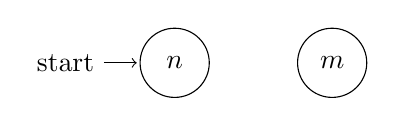
\begin{tikzpicture}[shorten >=1pt,node distance=2cm,on grid,auto]
% \tilkzstyle{every state}=[f
  \node[state,initial]  (n)                     {$n$};
  \node[state]          (m)    [right of = n]  {$m$};

%    <inital node> edge   node {label} (node_name)
%   (q)   edge        node {}     ()
%  \path[->]    %%TODO uncomment when PDFLATEX starts working to compile this lable
%    (n)  edge                node { $S_{1/0}:(L/R)$ }    (m);  %This is giving me an infinite compile time??
\end{tikzpicture}\\

ex: (These are the same)
$$Q_1S_1RQ_1,Q_1S_0S_1Q_2,Q_2S_1LQ_2,Q_2S_0RQ_3,Q_3S_1S_0Q_3,Q_3S_0RQ_4$$
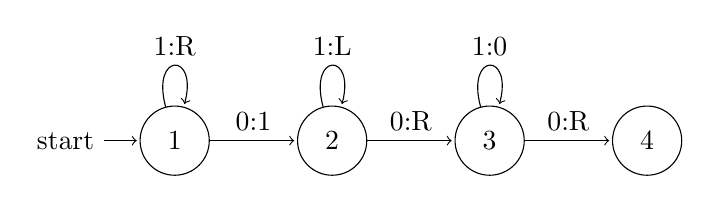
\begin{tikzpicture}[shorten >=1pt,node distance=2cm,on grid,auto]
% \tilkzstyle{every state}=[f
  \node[state,initial]  (1)                     {$1$};
  \node[state]          (2)    [right of = 1]   {$2$};
  \node[state]          (3)    [right of = 2]   {$3$};
  \node[state]          (4)    [right of = 3]   {$4$};

%    <inital node> edge   node {label} (node_name)
%ex:   (q)   edge        node {}     ()
  \path[->]
    (1)   edge  [loop above]  node    {1:R}   ()
    (1)   edge                node    {0:1}   (2)
    (2)   edge  [loop above]  node    {1:L}   ()
    (2)   edge                node    {0:R}   (3)
    (3)   edge  [loop above]  node    {1:0}   ()
    (3)   edge                node    {0:R}   (4);
\end{tikzpicture}\\

\begin{remark}[Turing Machines]
\begin{itemize}
\item Each Turing machine is a finite set of Turing instructions.
\item Each instruction is a 4 letter word of the Turing Alphabet.
\item The set of Turing machine is enumerable. (Proof: exercise)
%The set of 1 instruction turing machines is enumerable. (Map them to a two dimentional grid with X being inital states, Y being the final state, and the elements inbetween being the 8 combinations of operations of the two states. Then weave!
%For any n the set of n instruction Turing machines is also enumerbable.
%Use Induction!
%Then show the union of all this is enumerable.

%It could also be done with the number of states being enumerable.
\end{itemize}
\end{remark}

%Another lecture begins!
\begin{definition}[Standard inital configuration]
A Turing machine is in a standard Initial configuration $\iff$ 
\begin{itemize}
\item for some positive integer $k$, there are $k$ blocks of $1$'s on the tape. %Either there is just a single block of 1's, or two or three blocks of ones, and so-on
\item separated by a blank, %a single blank 
\item and the rest of the tape is blank. %or empty.
\item the machine is scanning the left-most $1$ on the tape.
\item the machine is in it's lowest numbered state.
\end{itemize}
ex: $\cdots0010110111000\cdots$ is a $SIC$. (if it's in lowest state)
ex: $\cdots00010000\cdots$ is a $SIC$.
\end{definition}


\begin{definition}[Standard final configuration]
A Turing machine is in a standard final configuration $\iff$ 
\begin{itemize}
\item there is a single block of $k$ $1$'s
\item and the rest of the tape is blank. 
\item the machine is scanning the left-most $1$ on the tape.
\end{itemize}
ex: $\cdots00111111000\cdots$ is a $SIC$. (if it's in lowest state)
ex: $\cdots00010000\cdots$ is a $SIC$.
\end{definition}


\begin{definition}[Computes a one-place function $f^1$]
A Turing $M$ computes a one-place function $f^1$: \\
if $M$ is started in a $SIC$ with a single block of $k$ $1$'s and
\begin{itemize}
\item if $f^1$ is defined for the argument $k$, then $M$ eventually halts in a $SFC$
\item or if $f^1$ is not defined for the argument $k$, then either $M$ never halts or it halts in a non-standard final configuration.
\end{itemize}
\end{definition}

\begin{remark}
Every Turing machine computes exactly one function of two arguments. %This is just because we can say it does, from how we defined it earlyer.
\end{remark}

\begin{remark}
For any $n$, each Turing Machine computes exactly one function of $n$ arguments.\\
The set of one-place Turing computable functions is enumerable \\
$\vdots$\\
The set of Turing computable functions is enumerable.
\end{remark}


%%Note: I missed a class, however I've eard there wasn't anything done last class


%Another lecture!
\begin{definition}[The halting problem]
The problem of finding an effective method to determine whether a Turing macine will eventually ahlt or not after it is started with some input.
\end{definition}
\begin{proof}[The halting problem is unsolvable]
Ex: $L_M: M_1,\dots$ \\
$h(m,n) =$ \\ % \left $ &  
%  $\begin{cases}
\quad 1 if $M_m$ eventually ahlts after starting with input $n$ \\
\quad 2 if $M_m$ never halts after starting with input $n$ \\ 
%$  \end{cases}$
The halting problem is solvable $iff$ $h$ is computable.
Show: $h$ is not Turing computable. \\
Let $C$ be a copying machine. \\
Let $F$ be $\frac{1}{2}$ flipper.\\
Suppose $h$ is Turing Computable.\\
Let $H$ be a Turing machine that computes $h$.\\
If $h$ is a Turing computable, then $H$ exists.\\
If $H$ exists, then $D(C-H-F)$ exists. \\
Let $D = M_k$, for some $k$. $M_k \in L_M$.\\
\\
Start $D$ with input $k$.
The C-part of $D$ will produce a copy of $k$,
Then the $H-$part will do its job:
\begin{itemize}
\item If $M_k$ will eventually halt after starting with input $k$, then $H$ will produce output $1$.
\item If $M_k$ will never halt after starting with input $k$, then $H$ will produce output $2$.
\end{itemize}
Then the $F-$part will do it's job.
\begin{itemize}
\item If output from $H$ is 1, $F$ will never halt.
\item If output from $H$ is 2, $F$ will eventually halt.
\end{itemize}
Giving us: \\
\begin{itemize}
\item If $M_k$ will eventually halt after starting with input $k$, then $D$ will never halt ater starting with input $k$. \\
\item If $M_k$ will never halt ater starting with input $k$, then $D$ will eventually halt after starting with input $k$. \\
\end{itemize}
So $M_k$ will halt, after starting with input $k$, $\iff$ $D$ will nver halt after starting with input $k$.\\
Then $M_k$ isn't identical with $D$, which is a contradiction! Hence$D$ doesn't exist. So $H$ does not exists. So $h$ is not turing computable.
\end{proof}


%% MORE LECTURE. YAY FEB 9, 2017.

\begin{proof}[Another halting problem..?]
$L_M: M_1, \cdots$
$L_F: F_1, \cdots$ \\
$g(n) = 1,$ if $f_n(n) = 2$ \\
$g(n) = 2,$ otherwise. \\
$g \not = f_k \forall k$ \\
$h(m,n)= 1 $if $M_m$ eventuall halys after starting with input $n$. \\
$h(m,n)= 2$ if $M_m$ never halts after starting with input $n$. \\
$s(m) = 1$, if $M_m$ eventually halts after starting with input $m$. \\
$s(m) = 2$, if $M_m$ never halts after starting with input $m$. \\
\begin{enumerate}
\item The halting problem is solvable iff $h$ is computable.
\item If $h$ is computable, then $s$ is computable.
\item If $s$ is computable, and $TT$'s is true, then $g$ is computable.
\item $g$ is not Turing computable.
\item Turing Thesis is true (Whatever is not Turing Computable is not computable)
\item The halting problem is not solvable.
\end{enumerate}
\begin{proof}[3.]
Suppose $S$ is computable and $TT$ is true. \\
Then: There is a Turing machine $S*$ that computes s.\\
Suppose that we are to calculate $g(n)$, for some $n$. \\
Start $S*$ with input $n$. \\
\begin{itemize}
\item Case 1: S* eventually halts with output 1\\
We know that $M_n$ will eventually ahlt after it is started with input $n$
Start $M_n$ with input $n$, when it halts, inspect the tape.
\begin{itemize}
\item Case 1.1: Halted in SFC
$f_n(n) = 2$ 
$g(n) = 1$
\item Case 1.2: Halted in non-SFC: $f_n$ is undefined.
$f_n(n) \not=2$
\end{itemize}
\large {
And then Blake broke it: \\
As it's a halting problem to figure out if it's in $SFC$?\\ }
\normalsize
$g(n)=2$
\item Case 2: S* eventually halts with output 2
We know that $M_n$ will never halt after it is started with input $n$. \\
So we know that $f_n$ is undefined for the argument $n$. \\
So we know that $g(n) = 2$ \\
\end{itemize}

\end{proof}
\end{proof}


%%Two weeks later: Some actual notes.. maybe. idk
%%Chapt 10 I think.
\section{Sentental logic}
Some symbols n things:
\begin{itemize}
\item ( 
\item ) 
\item Successor : ' %From the textbook anyways.
\item Not: -
\item And: $\wedge$ (Conjunction)
\item Or: $\vee$ (Disjunction)
\item Exists: $\exists$ 
\item Forall: $\forall$
\item Variables: $v_1, v_2, v_3, \dots$
\item Equality: $=$
\item Predicates: \begin{tabular}{c c c}
 $A^{1}_1$ & $A^{1}_2$  & \dots \\
 $\vdots $ & $\vdots$   & $\ddots$ \\
 $A^{n}_1$ & $A^{n}_2$  & $\dots$ \\
\end{tabular}
\item Constant names: $a_1, \dots$
\item Functions: \begin{tabular}{c c c}
 $f^{1}_1$ & $f^{1}_2$ & \dots \\
 $\vdots$    & $\vdots$ & $\ddots$ \\
 $f^{n}_1$ & $f^{n}_2$ & \dots \\
\end{tabular}
\end{itemize}


\begin{definition}[Term]
\begin{itemize}
\item Every variable is a(n atomic) (open) term.
\item Every constant is a(n atomic) (closed) term. %(or name?)
\item If $t_1,\dots,t_n$ are terms, then $f^n(t_1,\dots,t_n)$ is a term.  
\item Nothing else is a term.
\end{itemize}
\end{definition}

\begin{definition}[Formula]
\begin{itemize}
\item $A^n(t_1,\dots,t_n)$ is a formula where $A^n$ is an $n-$place predcate and $t_i$ are terms. (This is an atomic formula).
\item If $F$ is a formula then $-F$ is a formula
\item If $F$ and $G$ are fomulas then $(F\wedge G)$ is a formula.
\item If $F$ and $G$ are fomulas then $F(\vee G)$ is a formula.
\item If $F$ is a formula, then $\exists vF$ is a formula.
\item If $F$ is a formula then $\forall vF$ is a formula.
\item NOTHING ELSE IS A FORMULA.
\end{itemize}
\end{definition}


\begin{definition}[Bound]
%From lecture:
%An occurence of a variable $v$ in a formula $F$ is bound if it is in a part $G$ of $F$ where
%G = $\exists v \_\_\_\_\_\_\_$ or $G = \forall v \_\_\_\_\_\_\_\_\_\_\_\_\_.$

%From Textbook:
An occurrence of variable $x$ is bound if it is part of a subformula beginning $\forall x$ or $\exists x$, in which case the quantifier $\forall$ or $\exists$ in question is said to bind that occurrence of the variable $x$, and otherwise the occurrence of the variable $x$ is free. \\
Ex: $Fx \rightarrow \forall x F x$ : The first x is free, and the second is bound. \\
Ex: $x < y \wedge - \exists z ( x < z \wedge z < y )$: all occurrences of $x$ and $y$ are free, and all the occurrences of $z$ are bound.
\end{definition}

%Again, from the textbook:
\begin{remark}
When we write something like "Let $F(x)$ be a formula", we are to be understood as meaning "Let $F$ be a formula in which no variables occur free except $x$".
\end{remark}

%Still from the textbook:
\begin{definition}[Instance]
An $instance$ of a formula $F(x)$ is any formula of the form $F(t)$ for $t$ a closed term. Simmilar notations apply where there is more than one free variale, and to terms as well as formulas.
\end{definition}

%More textbook:
\begin{definition}[Sentence]
a formula is a sentence if no occurrence of any variable in it is free.
\end{definition}

%End: chapt-9.

%Chapt 10:
\begin{definition}[Model]
A model $M$ (interpretation) of a language $L$ is $\{|M| v\}$ Where $|M|$ is a non-empty set and $v$ is a valuation function that assigns values (extensions/denotations) to the mebers of $L$ in such a way that 
\begin{itemize}
\item $\forall v(a) \in |M|$
\item $v(A^n) \subseteq$ the $n$th caresian product of $|M|$ with itself: $|M|\cross \dots |M|$.
\item $v(f^n)$ is a total function from $|M| \cross \dots |M|$ to $|M|$.
\end{itemize}
\end{definition}


\begin{definition}[Truth]
\begin{itemize}
\item For some predicate $R$: $M \vDash R(t_1,\dots,t_n)$ iff $R^M(t_1^M,\dots,t_n^M)$ \\
\item For Identity function (when present): $M \vDash =(t_1,t_2)$ iff $t_1^M = t_2^M$.
\item $M \vDash F^n (t_1,\dots,t_n)$ iff $<M(t_1),\dots,M(t_n)> \in M(F^n)$. \\
Textbook writes this as: $(f(t_1, \dots t_n))^M = f^M (t_1^M , \dots, t_n^M)$.
Ie: Interpretation $M$, makes true $f^n(t_1,\dots,t_n)$ (An n-place function), iff $\{t_1^M , \dots, t_n^M\} \in M(F^n)$ %Is this correct? ben agrees 
%\item $M \vDash -S iff M \not = S$. %Notes
\item $M \vDash -S $ iff $M \not \vDash S$ %Textbook
%Textbook denotes K/L as F/G$.
\item $M \vDash (K \wedge L )$ iff $M \vDash K$ and $M \vDash L$ 
\item $M \vDash (K \vee L )$ iff $M \vDash K$ or $M \vDash L$ %From textbook
% Notes:
%\item $M \vDash \forall x F$
%\item $M \vDash \exists x F(c) iff $ there is an object $o \in |M| $ and given a name $c$ (that is not interpreted by $M$), $M: \vDash F(c)$
% Textbook: 
\item $M \vDash F[m]$ iff $M^c_m \vDash F(c)$ \\
'If we considered the extended language $L \cup \{c\}$ obtained by adding a new constant $c$ in to our given language $L$, and if among all the extentions of our given interpretation of this extended language we considered the one $M^c_m$ that assigns $c$ the denotation $m$, then $F(c)$ would be true.'

\item $M \vDash \forall x F (x) $ iff for every m in the domain , $M \vDash F(m)$
\item $M \vDash \exists x F (x) $ iff for some m in the domain , $M \vDash m)$

\end{itemize}
\end{definition}

\begin{definition}
of the denoteizan/extension of a closed term in a model M.
If $T$ is a name $M(t) = v(t)$
If $t$ is $f^n(t_1,\dots,t_n)$
then \\
$M(f^n(t_1,\dots,t_n)$
$M(f^n)(M(t_1),\dots,M(t_n)).$
\end{definition}

Validy = Satisfiability = Implication.\\

Misc-crap:
\begin{itemize}
\item $A \vDash B$ is $-(A \wedge -B)$
\end{itemize}

\begin{lemma}
Extensionality Lemma\\
\begin{itemize}
\item Let $M$ be a model of a language $L$.
\item Let $S$ be a sentence of $L$.
\item Let $L^+$ be an extension of $L$. $L \subseteq L^+$
\item Let $M^+$ be a model of $L^+$
\item So: $M^+$ is an extension of $M$.
\item $M \vDash S$ iff $ M^+ \vDash S$
\end{itemize}
\end{lemma}
Example:

If $A \vDash B$ and $B \vDash C$, then $A \vdash C$.
Suppose $A \vDash B$, and $B \vDash C$.\\
In every interpretation of $A$ and $B$ in which $A$ is true, $B$ is true,
In everry interpretation of $B$ and $C$ in which $B$ is true, $C$ is true.
Shows: In every interpretation of $A$ and $C$ in which $A$ is true, $C$ is true.

Let $M$ be an interpretation of $A$ and $C$ such that $M \vDash A$.
\begin{itemize}
\item Case 1:
$M$ is an interpretation of $B$. \\
Then $M \vDash B$ \\
So $M \vDash C$. \\
\item $M$ is not an interpretation of $B$. \\
Then there is an extension $M^+$ that interprets $B$ as well as $A$ and $C$. \\
so: $M^+ \vDash B$ \\
So: $M^+ \vDash C$ \\
So $M \vdash C$ (By the ext, llemma) \\
\end{itemize}


%Stuff I kinda missed.
\begin{lemma}[Undecibality]
If the decision problem (for implication) is solvable, then the halting problem is solvable.
There is an effective methoid for specifiing for any Turing machine $M$ and any input $N$ a finite set of setences $\Delta$ and a sentence $H$ such that $\Delta \vDash H$ iff $M$ eventually halts after starting with input $n$. \\
$\Delta \vDash H$ iff $M$ eventualy alts after start with input n.\\


%\begin{proof}
Define the one place predicate $Q_ij$ as: At time $j, M$ is in state $i$.
Define the two place preidcate $@js$ as At time $j, M$, is scanning square $s$.
Define the two place predicate $Mjs$ as: At time $j,$ square $s$ is marked with a $1$.

A description $D$ for a start state could then be:
$D: [Q_10 \wedge @_{0,0} \wedge M_{0,0} \wedge M_{0,1} \wedge M_{0,2} \wedge \forall y((y \not = 0 \wedge y \not = 1 \wedge y \not = 2 ) \implies - M_{0,y}]$
Time = 0, $[ \dots 0 1 1 1 0 \dots ]$
Square \#, $[\dots -1 0 1 2 3 \dots ]$

%\end{proof}
\end{lemma}

%Some examples n stuff here.
For each instructon of a $TM$, we may write the instruction as a setence: \\
$Q_{i1}S_1RQ_{i2}$ : 
Move right seeing 1 in state: \\
%Note: these are fome someone elses notes, and syntax may be wrong.
$\forall x \forall t ((Q_{i,1} \wedge @_{t,x} \wedge M_{t,x}) \implies (Q_{i2,(t+1)} \wedge @_{(t+1),(x+1)} \wedge \forall y((M_{t,y} \implies M_{(t+1),y}) \wedge (- M_{t,y} \implies - M_{(t+1),y}))$


%New lecture:
Misc-crap that's on the board for some reason: \\
%Seems like shorthand for definitions... and something about Delta.
\begin{align*}
 & \Delta \\
\mathbb{Q}^1_2  &:& \forall x \forall y \forall z ((Sxy \wedge Sxz) \implies y = z)       & \text{}\\
@^2            &:& \forall x \forall y \forall z ((Sxz \wedge Syz) \implies x = y )       & \text{}\\
M^2             &:& \forall x \forall y ( Sxy \implies x < y )                            & \text{}\\
0               &:& \forall x \forall y \forall z ((x < y \wedge y < z ) \implies x < z ) & \text{}\\
S^2             &:& - \exists x , x < x                                                   & \text{+1}\\
<^2             &:& & \text{lessthan}
\end{align*}

Some thingelse now too:\\
%Node 1 : 1:R -> node 2
$\forall x \forall t ((Q_1 t \wedge @tx \wedge Mtx ) \implies \exists u ( s_1 (t , u) \wedge Q_2(u) \wedge @ (u,v)) \wedge \forall y ((M(t,y) \implies M(u,y)) \wedge (-M(t,y) \implies - M(u,y)))))$ \\
$\exists x \exists t ( Q_mt \wedge @tx \wedge Mtx)$\\


\begin{proof}
Something about biconditonal:\\
$\Delta \vDash H$ iff $M$ halts after starting with input n.
\begin{enumerate}
\item if $\Delta \vDash H$, then $M$ halts.
\item if $M$ halts, then $\Delta \vDash H$.
\end{enumerate}
\begin{enumerate}
\item if $\Delta \vDash H$, then $M$ halts - Proof. \\
Suppuse $\Delta \vDash H$ \\
All members of $\Delta$ are true in the standard interpretation I.
$H$ is true in $I$.
So: $M$ halts.
\item if $M$ halts, then $\Delta \vDash H$ - Proof. \\
Suppose $M$ halts. (Show $\Delta \vDash H$). \\
There is a time \underline{$t$} $M$ halts at t. \\
There is a state $q_i, M$ halts at $t$ in state $q_i$. \\
There is a square $x$, $M$ halts at $t$ in state $q_i$, scanning square $x$ which is Marked / $-$ Makred \\
1: $Q_i(t) \wedge @(t,x) \wedge M(t,x)$. \\
%These ones are names
1 is a cojunct of the description of time t, $\mathbb{D}(t)$ \\
$\mathbb{D}(t) \vDash (i)$ \\
%consider now..

2: $\exists x \exists t (Q_1(t) \wedge @ (t,x) \wedge (t,x))$. \\
%These ones are variables.

$(i) \vDash (ii)$. \\
$(ii)$ is disjunct of $H$. \\
$(ii) \vDash H.$ \\
So: $\mathbb{D}(t) \vDash H$. \\

%D: the discription at time $t.

$\Delta$ implies a description of everytime before which $M$ did not halt. \\
$\forall n$( if $M$ has not halted before time n, then $\Delta \vDash \mathbb{D}(n)$ \\
\end{enumerate}
\end{proof}


%ANOTHER LECTURE Tue Mar 14.
Relisting it: 
\begin{proof}[The decision problem for implication, is unsovable if turings thesis is true.]
$\Delta \vDash H$ iff $M$ eventually halts. \\
Only if: $\Delta \vDash H$ only if $M$ eventually halts. \\
if: if $M$ eventually halts then $\Delta \vDash H$. \\
Suppose: $M$ halts at $t$\\
$\mathbb{D}(t) \vDash(H)$ \\ %Proved earlyer?
Show: $\Delta \vDash \mathbb{D}(t)$

Something inductive:
Base step: if $M$ has not halted before time 0, then $\Delta \vDash \mathbb{D}(0)$:
Inductive step: $\forall n ($ if $M$ has not halted before time $n$, then $\Delta \vDash \mathbb{D}(n)$ only if if$M$ has not halted before time $n+!$, then $\Delta \vDash \mathbb{D}(n+1))$
% Induction layout:
% F_0
% \forall n (F_n \implies F_{n+1}
% \forall n F_n
Conclusion: $\forall n$ (if $M$  has not halted before time $n$, then $\Delta \vDash \mathbb{D}(n)$.

Proving the Inductive step: \\
\begin{itemize}
\item Suppose if $M$ has not halted before time $n$, then $\Delta \vDash \mathbb{D}(n)$.
\item (Show : if $M$ has not halted before time $n+!$, then $\Delta \vDash \mathbb{D}(n+1)$)
\item Suppose: $M$ has not halted before time $n+1$
\item So: $M$ has not halte dbefore time $n$
\item So: $\Delta \vDash \mathbb{D}(n)$.
\item (Show: $\Delta \cup \{\mathbb{D}(n)\} \vDash \mathbb{D}(n+1))$
\item $\mathbb{D}(n): Q_jn \wedge @_{n,k} \wedge M_{n,k} \dots$
\item $\forall t \forall x ((Q_j(t) \wedge @tx, \wedge Mtx) \implies Q_it+1 \wedge @(t+1)(x+1) \wedge \dots)$
\item $(Q_jn \wedge @nk \wedge Mnk) \implies Q_i(n+1) \wedge @(n+1)(k+1) \wedge \dots)$
\item $\mathbb{D}(n+1): Q_i(n+1) \wedge @(n+1)(j+1)\wedge \dots$
%How do you write this out? HAha, you should kow this already. apprently. idfk wtf he's on about.
%There are 3 cases: move left, move right, write somthing. And that in each case, prove the conclusion thingy.
\end{itemize}

\end{proof}

Then some random ramblings about logiceans. happend. Here's a book: "What is the name of this book?".\\
There are methods of validlity, and truth trees, and some other stuff. He's gonna use this. He's gonna prove this has some properties for validity. \\

\section{Truth Trees}
Ex:
$\frac{(A \implies B) \\ A}{B}$ 
\hspace*{2cm} IS
%Tree: \\
%$(A \implies B)$ \\
%$A$ \\
%$-B$ \\
%left subnode: $-A$
%Right node :$B$
\begin{prooftree}
{
  to prove={A \implies B}
}
  [A , just=Assummed
    [-B, 
      [-A, close={!u,!c}]
      [B, close={!u,!c}]]]]
\end{prooftree}

Giving
$\{ ( A \implies B) , A , -B \}$ \\
%Example LATEX proof-tree:
%\begin{prooftree}
%{
%  to prove={\{P \vee (Q \vee \lnot R), P \rightarrow \lnot R, Q \rightarrow \lnot R\} \vdash \lnot R}
%}
%  [P \vee (Q \vee \lnot R), just=Ass, checked
%    [P \rightarrow \lnot R, just=Ass, checked
%      [Q \rightarrow \lnot R, just=Ass, checked, name=last premise
%        [\lnot\lnot R, just={$\lnot$ Conc}, name=not conc
%          [P, just={$\vee$ Elim:!uuuu}
%            [\lnot P, close={:!u,!c}]
%            [\lnot R, close={:not conc,!c}, just={$\rightarrow$ Elim:!uuuu}]]
%          [Q \vee \lnot R
%            [Q, move by=1
%              [\lnot Q, close={:!u,!c}]
%              [\lnot R, close={:not conc,!c}, just={$\rightarrow$ Elim:last premise}]]
%            [\lnot R, close={:not conc,!c}, move by=1, just={$\vee$ Elim:!u}]]]]]]
%\end{prooftree}


%\large{First-Order Logic Revamp:}
%From Chapt. 9:
%Some definitions for first-order logic: \\
%\begin{itemize}
%\item Logical Symbols: \\
%\begin{itemize} 
%\item Negation: ~ : 'not'
%\item Conjunction: \&, $\wedge$: 'and'
%\item Disjunction: $\vee$ : 'or'
%\item Conditional: $\rightarrow$ : 'if \dots then \dots'
%\item Biconditional: $\leftrightarrow$ : 'if and only if'
%\item Universal quantification: $\forall x$ : 'for every x'
%\item Existential quantification: $\exists x$ : 'for some x'
%\item Identity symbol: $=$ : '\dots is (the very same thing as ) \dots'
%\item Variables: x, y, z
%\item Punctuation: '(', ')' , ','
%\end{itemize}
%\item Nonlogical Symbols:
%\begin{itemize}
%\item Constants or Individual symbols (a,b,c .. )
%\item Predicates or Relation symbols : Have a fixed positive number of places
%\item Function symbols: : Have a fixed positive number of places.
%\end{itemize}
%%End-Symbols
%\item Other-Definitions:
%\begin{itemize}
%\item language: an enumerable set of nonlogical symbols. Denoted: $L$ \\
%Empty Language: $L_\varnothing$, The language with no logical symbols.
%\end{itemize} %End-other defintions
%
%\item Closure:
%\begin{itemize}
%\item Closed Function: they make a complete statement capable of being true or false
%\item Closed Term: Has no variables.
%\end{itemize}
%
%\item Interpretation: An interpretation $M$ for a language $L$ consists of two components.
%\begin{itemize}
%\item A nonempty set $|M|$, called the domain or universe of discourse of the set of things $M$.
%\item For each non-logical symbol, a denotation assigned to it. Noted by $x^M$.
%\end{itemize} %End Interpretations
%
%\end{itemize} %end some defs for first-order logic.
%

\newpage

\end{document}
